\section{Introduction}

Storage tracing and analysis has a long history.  Some of the earliest
filesystem traces were captured in 1985~\cite{ousterhout85}, and there
has been intermittent tracing effort since then, summarized by
Leung~\cite{LeungUsenix08}.  These traces are
analyzed to find properties that future systems should support or
exploit, and as input to simulators and replay tools to explore system
performance with real workloads.

One of the problems
with trace analysis is that old traces inherently have to be scaled up
to be used for evaluating newer storage systems because the
underlying performance of the newer systems has increased.  Therefore,
the community benefits from regularly capturing new traces from multiple
sources, and if possible, traces that put a heavy load on the storage
system, reducing the need to scale the workload.

Most traces, since they are performed by academics, are captured in
academic settings.  This means that the workloads captured are
somewhat comparable, but it also means that commercial workloads are
under-emphasized.  Microsoft is working to correct this by capturing
commercial enterprise traces from their internal
servers~\cite{snia-iotta-microsoft}.  Our work focuses on commercial
NFS~\cite{rfc1094nfs,rfc1813nfsv3,Pawlowski94nfs3} workloads, in particular from a feature animation (movie) company.
The name of the company remains blinded as part of the agreement to
publish the traces.  The last publically available NFS traces that we
are aware of were collected in 2003.  Our 2003 and 2007
traces~\cite{animation-bear-traces} provide recent NFS traces for use
by the community.

One difference between our traces and other ones is the data rates
that we measured.  Our 2003 client traces saw about 750 million
operations per day.  In comparison, the 2003 Ellard
traces~\cite{EllardLisa03} saw a peak of about 125 million NFS
operations per day, and the 2007 Leung traces~\cite{LeungUsenix08}
saw a peak of 19 million CIFS operations/day.  Our 2007 traces saw
about 2.4 billion operations/day.  This difference required us to
develop and adopt new techniques to capture, convert, and analyze the
traces.

Since our traces were captured in such a different environment than
prior traces, we limit our comparisons to their workloads, and we
do not attempt to make any claims about trends.  We believe that
unless we, as a community, collect traces from hundreds of different
sites, we will not have sufficient data to make claims stronger than
``this workload is different from other ones in these ways.''  In
fact, we make limited comparison in the trends between our 2003 and
2007 traces for similar reasons.  The underlying workload changed
as the rendering techniques improved to generate higher quality output,
the operating system generating the requests changed, the NFS
protocol version changed, and the configuration of the clients 
changed because of standard technology trends.

The process of understanding a workload involves four main
steps, as shown in Figure~\ref{fig:overall-process}.  Our tools for
these steps are shown in italics for each step, as well as some
traditional tools.  The first step is capturing the workload, usually
as some type of trace.  The second step is conversion, ususally from
some raw format into a format designed for analysis.  The third step
is analysis to reduce the huge amount of converted data to
something manageable.  Alternately, this step is a simulation or replay to
explore some new system architecture.  Finally the fourth step is to
generate graphs or textual reports from the output of the analysis or
simulation.

Our work has five main contributions:

\begin{enumerate}
\item The development of techniques for lossless raw packet capture up to
5Gb/s, and with the hardware improvements since our work, likely to
10Gb/s.  These techniques are applicable to anyone wanting to capture
a network storage service such as NFS, CIFS, or iSCSI.

\item A series of guidelines for the conversion and storage of the
traces.  Many of these guidelines are things that we wish we had known
when we were converting our traces.  We used
DataSeries~\cite{DataSeriesOSR2009} to store the traces, but our
guidelines are general.

\item Improved techniques for analyzing very large traces that allow
us to look at the burstiness in workloads, and an examination of how
the long averaging intervals in prior analysis can obscure workload
properties.

\item The analysis of an intense NFS workload demonstrating that our
techniques are successful.

\item The agreement with the animation company to allow the roughly
100 billion operation anonymized traces to be published, along with
the complete set of tools to perform all the analysis presented in
this paper and to generate the graphs.  Other
researchers can build on our tools for further analysis, and use
the traces in simulation studies.
\end{enumerate}

\begin{figure}
\center 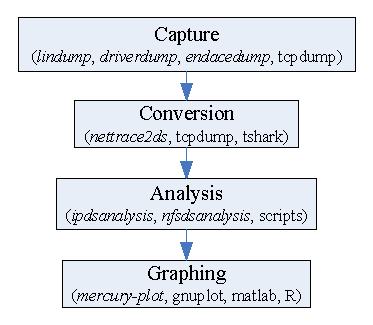
\epsfig{width=2.2in, angle=0, file=overall-process.eps}
\caption{Overall process; our tools are shown in italics, traditional tools
after them.}
\label{fig:overall-process}
\end{figure}

We examine related work in section~\ref{sec:related}.  We describe our
capture techniques in section~\ref{sec:capture}, followed by the
conversion (section~\ref{sec:conversion}). We describe our adopted and
new analysis techniques in section~\ref{sec:analysis-techniques} and
use them to analyze the workload in section~\ref{sec:analysis}.
Finally we conclude in section~\ref{sec:conclusion}.
